%%%%%%%%%%%%%%%%%%%%%%%%%%%%%%%%%%%%%%%%%%%%%%%%%%%%%%%%%%%%%%%%%%%%%%%%%%%%%%%%%%%%%%%%%%%%%%%%%%%%%%%

\documentclass[prb,aps,12pt,superscriptaddress,floatfix]{revtex4-2} 
\usepackage{graphicx}
\usepackage{color} 
\usepackage{amsmath}
\usepackage{amssymb} 
\usepackage{natmove}
\usepackage{natbib}
\usepackage{hyperref} 
\usepackage{bm}

%%%%%%%%%%%%%%%%%%%%%%%%%%%%%%%%%%%%%%%%%%%%%%%%%%%%%%%%%%%%%%%%%%%%%%%%%%%%%%%%%%%%%%%%%%%%%%%%%%%%%%%

\begin{document}

\title{\huge Shrimpoluminescence}

\author{\large Tyler C. Sterling}
\email{ty.sterling@colorado.edu}
%\affiliation{Department of Physics, University of Colorado at Boulder, Boulder, Colorado 80309, USA}

\date{\today}

%\begin{abstract}
%    abstract
%\end{abstract}

\maketitle

%\listoffigures
%\listoftables
%\tableofcontents

%%%%%%%%%%%%%%%%%%%%%%%%%%%%%%%%%%%%%%%%%%%%%%%%%%%%%%%%%%%%%%%%%%%%%%%%%%%%%%%%%%%%%%%%%%%%%%%%%%%%%%%

\begin{figure}
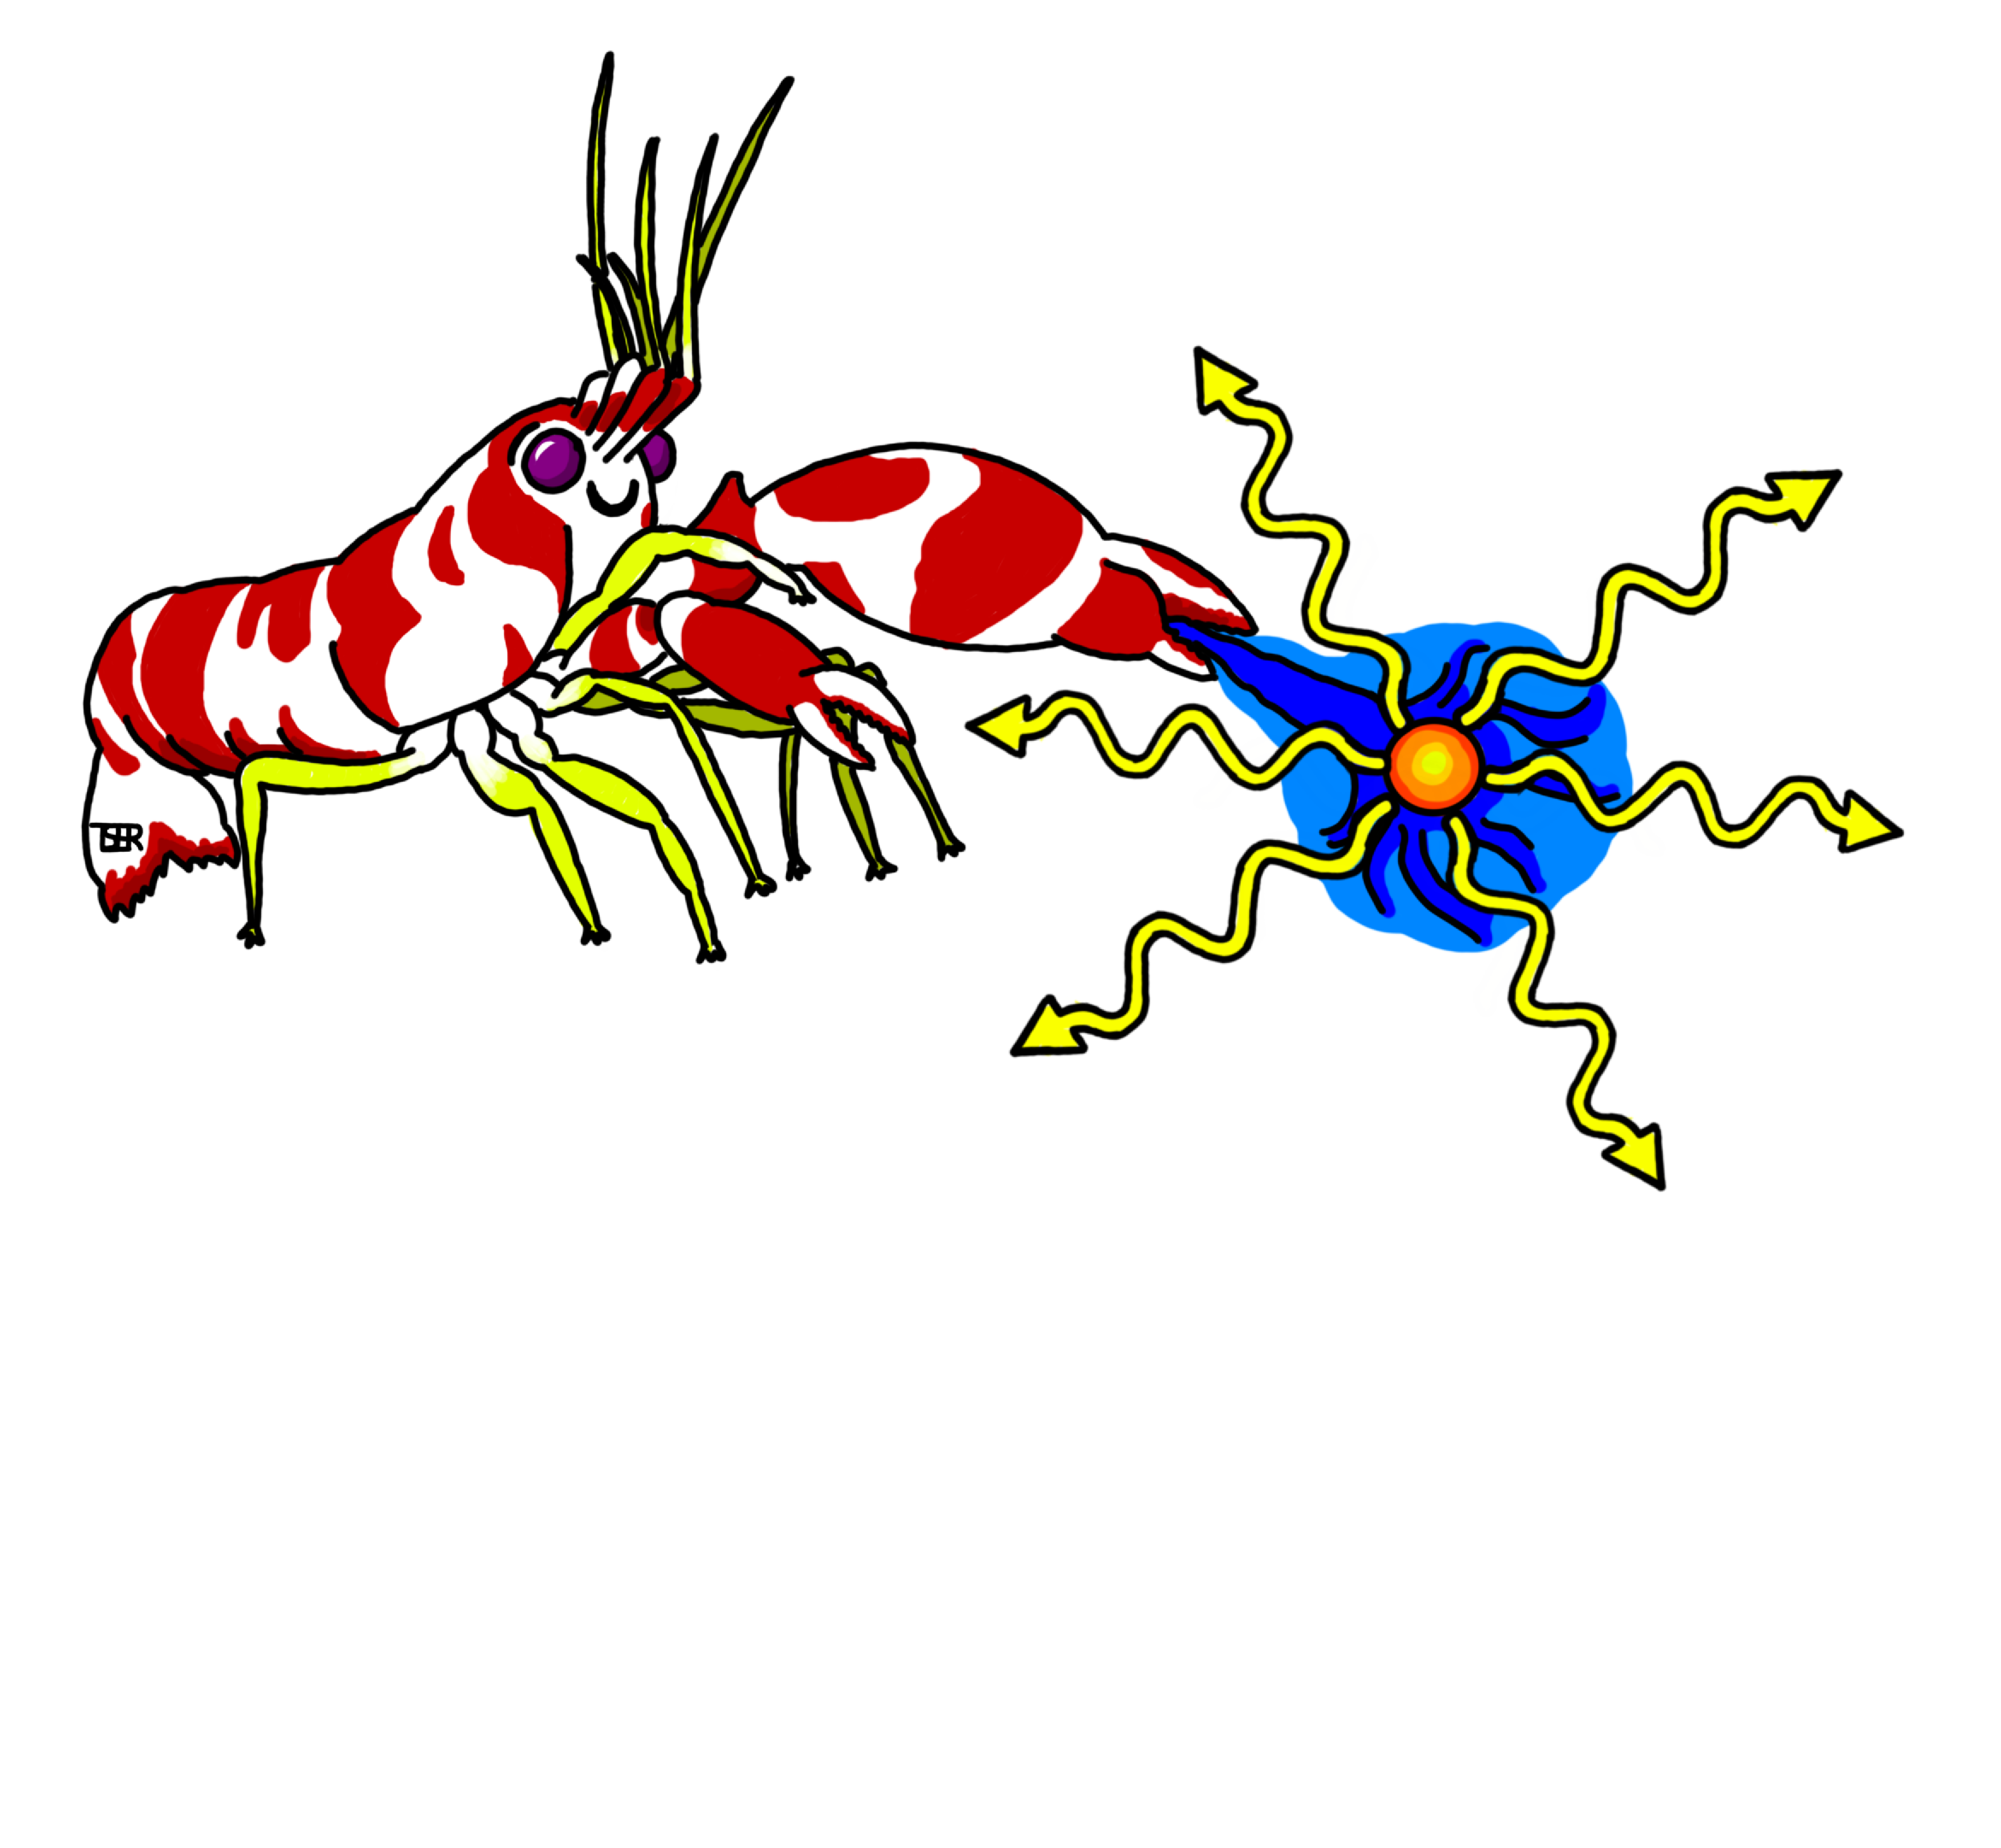
\includegraphics[width=1\linewidth]{figs/shrimpy.pdf}
%    \caption{}
\label{fig:shrimpy}
\end{figure}

 
\newpage

\section{Details of the project}
Pistol shrimp, like the red-banded pistol shrimp shown in Fig. \ref{fig:shrimpy}, are capabale of generating a jet of water with high enough velocity that a \emph{cavitation} bubble forms behind it. When the bubble collpases under the pressure of the sea, enough energy is released to produce a shock-wave that can kill the shrimp's prey \cite{}. If the shrimp's prey had very sensitive eyes (and also weren't dead) they might also see a flash of light produced through an effect referred to as ``shrimpoluminescence" in the case of the pistol shrimp, but more generally known as \emph{sonoluminescence} \cite{}.

\section{Paper Topic}

Some items to consider in the introduction of the actual paper. Caviation bubbles capabale of sonoluminesce occur in numerous places in nature:
\begin{itemize}
    \item the snapping and mantis shrimps us caviation bubbles to create shock waves that kill prey
    \item cavitation bubbles occur in pumps and after propellers and the shock damages the machinery
    \item ...
\end{itemize}




%%%%%%%%%%%%%%%%%%%%%%%%%%%%%%%%%%%%%%%%%%%%%%%%%%%%%%%%%%%%%%%%%%%%%%%%%%%%%%%%%%%%%%%%%%%%%%%%%%%%%%%

\bibliography{ref}

\end{document}
